\documentclass[12pt,          % font size: 11pt or 12pt
               phd,           % degree:    ms or phd
               onehalfspacing % spacing: onehalfspacing or doublespacing
               ]{ncsuthesis}

%%----------------------------------------------------------------------------%%
%%------------------------------ Import Packages -----------------------------%%
%%----------------------------------------------------------------------------%%

\usepackage{booktabs}  % professionally typeset tables
\usepackage{amsmath}
\usepackage{textcomp}  % better copyright sign, among other things
\usepackage{xcolor}
\usepackage{lipsum}    % filler text
\usepackage{longtable}
%\usepackage{subfig}    % composite figures
%\usepackage{natbib}    % ability to use citet,citep
\usepackage[backend=biber, natbib=true, style=apa]{biblatex}
\addbibresource{StudentName-thesis.bib}
%\usepackage{fancyhdr}  % creates headers
%\pagestyle{fancy}


%%---------------------------------------------------------------------------%%
%%  Bibliography 
%% or use BibTeX
%\bibliography{StudentName-thesis}
%% \bibliographystyle{apalike}


% Citations should be of the form ``author year''  not ``author, year''
% \bibpunct{(}{)}{;}{a}{}{,} % changes apalike bst into AMS format
 
%%----------------------------------------------------------------------------%%
%%---------------------------- Formatting Options ----------------------------%%
%%----------------------------------------------------------------------------%%
%%

%% -------------------------------------------------------------------------- %%
%% Disposition format -- any titles, headings, section titles
%%  These formatting commands affect all headings, titles, headings,
%%  so sizing commands should not be used here.
%%  Formatting options to consider are
%%     +  \sffamily - sans serif fonts.  Dispositions are often typeset in
%%                    sans serif, so this is a good option. 
%%     +  \rmfamily - serif fonts
%%     +  \bfseries - bold face
%\dispositionformat{\sffamily\bfseries}   % bold and sans serif
\dispositionformat{\bfseries}            % bold and serif

%% -------------------------------------------------------------------------- %%
%% Formatting for centered headings - Abstract, Dedication, etc. headings
%%  This is where one might put a sizing command.
%%  \MakeUppercase can be used to typeset all headings in uppercase.
\headingformat{\large\MakeUppercase}   % All letters uppercase
%\headingformat{\large}                % Not all uppercase
%\headingformat{\Large\scshape}        % Small Caps, used with serif fonts.

%% Typographers recommend using a normal inter-word space after
%% sentences. TeX's default is to add an wider space, but \frenchspacing
%% gives a normal spacing. Comment out the following line if you prefer wider spaces between sentences.
\frenchspacing

%% -------------------------------------------------------------------------- %%
%%  Optional packages
%%    A number of compatible packages to improve the look and feel of
%%    your document are available in the file optional.tex 
%%    (For example, hyperlinks, fancy chapter headings, and fonts)
%% To use these options, uncomment the next line and see optional.tex
\include{optional}
%solve bug from fancyhdr in optional
%http://nw360.blogspot.com/2006/11/latex-headheight-is-too-small.html
%\setlength{\headheight}{26.94345pt} % corrected error in Overleaf
%\fancyhead[L]{\vspace{1mm}} % only puts chapter title in headers

%%----------------------------------------------------------------------------%%
%%---------------------------- Content Options -------------------------------%%
%%----------------------------------------------------------------------------%%
%% Size of committee: 3, 4, 5, or 6 -- this number includes the chair
\committeesize{5}

%% Members of committee
%%  Each of the following member commands takes an optional argument
%%   to specify their role on the committee.
%%  For co-chairs, use the commands:
%%      \cochairI{Doug Dodd}
%%      \cochairII{Chris Cox}
%%
\chair{Rubén Rellán Álvarez}
\memberI{Rubén Rellán Álvarez}
\memberII{James Holland}
\memberIII{Jun Ying Tzeng}   % unnecessary if committeesize=3
\memberIV{Rafael Guerrero}    % unnecessary if committeesize=3, 4

%% Student writing thesis, \student{First Middle}{Last}
\student{Fausto Villafrade}{Rodríguez Zapata} % a full middle name

%% Degree program e.g. Marine, Earth, and Atmospheric Science
\program{Genetics}

%%!!!!!! To Change Year !!!!!!%%
% If year of graduation is not same as current year (common for December graduates
% thanks to the Grad Schools odd graduation rules) go into ncsuthesis.cls and change 
% \the\year in the line:
% \newcommand{\ncsu@year}{\the\year}
% to the year of graduation. E.g.:
% \newcommand{\ncsu@year}{2020}

%% Thesis Title
%%  Keep in mind, according to ETD guidelines:
%%    +  Capitalize first letter of important words.
%%    +  Use inverted pyramid shape if title spans more than one line.
%%
%%  Note: To break the title onto multiple lines, use \break instead of \\.
%\thesistitle{A North Carolina State University Sample \LaTeX{} Thesis \break 
%with a Title So Long it Needs a Line Break}
\thesistitle{Genomic Insights on Maize Local Adaptation to Low Phosphorus Availability}

%% Degree year. Necessary if your degree year doesn't equal the current year.
%\degreeyear{1995}

%% While your here make sure to change the PDF characteristics in optional.tex!!!

%%----------------------------------------------------------------------------%%
%%---------------------------- Personal Macros -------------------------------%%
%%----------------------------------------------------------------------------%%

%% A central location to add your favorite macros.

%% A few examples to get you started.
\newcommand{\uv}[1]{\ensuremath{\mathbf{\hat{#1}}}}
\newcommand{\bo}{\ensuremath{\mathbf{\Omega}}}
\newcommand{\eref}[1]{Eq.~\ref{#1}}
\newcommand{\fref}[1]{Fig.~\ref{#1}}
\newcommand{\tref}[1]{Table~\ref{#1}}

%% Add commonly used words
\newcommand{\mex}{\textit{mexicana}\xspace}
\newcommand{\hpc}{\textit{HPC1}\xspace}
\newcommand{\parv}{\textit{parviglumis}\xspace}

%% code inline frormatiing 
\newcommand{\code}{\texttt}

%%---------------------------------------------------------------------------%%
\begin{document}
%%---------------------------------------------------------------------------%%
\frontmatter

%% ------------------------------ Abstract ---------------------------------- %%
\begin{abstract}

In \autoref{chap-one} I use genome scans in traditional varieties, and QTL linkage mapping in a biparental population to explore the role of phospholipid metabolism in maize adaptation to highlands. 
Comparing highland and lowland maize populations I found evidence of selection in leaf phosphatidylcholine (PC) and lysophosphatidylcholine (LPC) composition; and in the sequence of genes coding for phospholipid metabolism enzymes. 
Using Recombinant Inbred Lines (RILs), I mapped an increased PC content, and PC/LPC ratio to the \hpc (\textit{High Phosphatidylcholine 1}) locus.
 \hpc is a predicted phosphoplipase A with orthologs that catalyze the degradation of PCs into LPCs. 
Consistent with a role in PC degradation
\hpc CRISPR-Cas9 mutants accumulated PCs like the plants carrying the highland allele.
Furthermore, the highland allele in \hpc was introgressed from highland teosinte \textit{Zea mays spp. mexicana} and is associated with earlier flowering in Mexican traditional varieties and temperate inbreds.
The marked gene-by-environment, $ G\times E $, interaction shown by \hpc points to its role in local adaptation to highlands, where the highland allele speeds up flowering while delaying it in the lowlands.
Further biochemical characterization suggests a mechanism by which the highland \hpc variant interferes with the flowering signaling pathway, by shifting the composition of leaf lipids binding to the \textit{FT} ortholog in maize \textit{ZCN8}.

Similar to \hpc, the chromosomal inversion \invfour also shows a $G \times E$ interaction effect on flowering time congruent with local adaptation to highlands, where it has been introgressed into cultivated maize from teosinte \mex too.

In \autoref{chap-three} I tested whether \invfour-highland contributes to local adaptation through an enhanced phosphorus starvation response (PSR). 
First, we bred Near Isogenic Lines (NILs) in B73 containing \invfour-highland introgressed from Mi21, a traditional Mexican maize variety, isolating the effect of \invfour-highland in a single genetic background.
Then we grew the \invfour-highland and control lines in the field under phosphorus sufficiency and deficiency. 
We measured flowering time, plant morphology, and leaf gene expression with RNA-seq. We found that independent of soil phosphorus status, \invfour-highland NILs flowered faster and grew taller than the controls while maintaining grain yield. 
There was a genomewide transcriptomic response to available phosphorus, affecting 7373 differentially expressed genes (DEGs), with the largest effect shown by the PSR regulator \textit{PILNCR1-miR399} . 
The effect of \invfour-highland is narrower, affecting 528 DEGs, mainly within the boundaries of the inversion.
The \invfour perturbation of PSR is limited to the putative aldehyde dehydrogenase \textit{aldh2}. 
Our results confirm the contribution of \invfour to faster flowering, but we don’t find evidence of its effect on PSR.

Because of their volcanic composition, andosols have high phosphorus content, but most of it is retained by vitreous minerals and is not available for plants.
Acrisols, with a sedimentary composition, have a high clay content and show low phosphorus availability as well. 

In \autoref{chap-four}, I search for genetic determinants of kernel mineral accumulation in a population derived from plants bred in these two different phosphorus-limited soils. 
First, we generated BC$_2$S$_3$ maize RILs of Mexican andosol donors backcrossed into CML530, a tropical inbred selected in Colombian acrisol.
From these, I obtained kernel concentrations for 14 minerals from plants grown under phosphorus sufficiency.
Here I detected 12 quantitative trait loci for 7 minerals, explaining between 1.8 to 17\% of the observed variance.
Two overlapping QTL peak intervals, for phosphorus and manganese, include \textit{Zm00001eb076150} a maize homolog of \textit{WAT1}, an auxin transporter in \textit{Arabidopsis}.
In low phosphorus conditions \textit{Zm00001eb076150}, has been previously associated with leaf number in maize and shoot dry weight in wheat. Linkage to this auxin transporter suggests a role for it in differential kernel phosphorus accumulation.

\end{abstract} 



%% ---------------------------- Copyright page ------------------------------ %%
%% Comment the next line if you don't want the copyright page included.
\makecopyrightpage

%% -------------------------------- Title page ------------------------------ %%
\maketitlepage

%% -------------------------------- Dedication ------------------------------ %%
\begin{dedication}
 \centering To my parents.
\end{dedication}

%% -------------------------------- Biography ------------------------------- %%
\begin{biography}
% The author was born in a small town \ldots
Born in Bogotá, Colombia in 1981 to Luz María Zapata Gamba and Lino Rodríguez.
Thanks to the courage of my mother and the support of all my family, I was able to secure scholarships ever since my high school education at Instituto Alberto Merani (1997, funded by B'nai Brith support). 
Later I graduated with a Bachelor of Science degree in Biology at Universidad de Los Andes, Colombia (2005, Neme Foundation and 50 years Fund Scholarships).
I started my work in plant genetics, genomics, and bioinformatics in QTL mapping of fungal disease resistance genes in common bean at CIAT (International Center for Tropical Agriculture, Cali) where I completed my thesis project under the direction of Dr. Joe Tohme.
This way I managed to be the first university graduate in my family.
I stayed at CIAT as a research assistant until 2012 where I published collaborations on the cassava genome, abiotic stress gene expression, and microRNA annotation.
In 2016 I completed my Ms. Sc. Degree in Biological Sciences at Universidad de Los Andes, Colombia (with a Graduate Studies Scholarship for Academic Excellence) under the direction of Dr. Santiago Madriñán Restrepo, where I studied the possibility of using nuclear DNA content quantification and leaf morphology to trace evidence of interspecies hybridization in the coca plant (\textit{Erythroxylum sp.}).
In 2019 I started my doctoral work in the "Genetics, Evolution and Metabolism of Maize Adaptation Lab" under Dr. Rubén Rellán Álvarez supervision at the North Carolina State University. 
Here I conducted my research on the genetics of maize adaptation to the Mexican Highlands thanks to the auspicious funding of the State of North Carolina (from the NCSU Graduate Student Support Plan, GSSP) and the Federal Government of the United States (from the NSF Science and Technologies for Phosphorus Sustainability, as a STEPS Scholar).
\end{biography}

%% ----------------------------- Acknowledgements --------------------------- %%
\begin{acknowledgements}
Thanks to the native peoples and farmers that domesticated, cultivated and bred maize. 
To all the maize genetics community and the people whose work made mine possible. 

Thanks to the support of my family: 
my mother Luz María Zapata Gamba, my father Lino Rodríguez, my sisters Andrea del Pilar and Ana Bolena, and my nieces Lina Fernanda and Luciana.
The main reason that I could ever achieve the dream of being a scientist.

Thanks to Dr. Rubén Rellán Álvarez, for his endless support, advice, and invaluable friendship.
An extraordinarily dedicated scientist and the most generous person I know.

Thanks to Dr. Allison Barnes, for her friendship, her openness, and all her determination required to get stuff-done and running the lab smoothly.

Thanks to the other members of my committee for their feedback and patience,  and for believing in me even when I did not. 
To Dr. Jim Holland for his constructive criticism and keen comments, for all the population genetics he taught me, and for having the good judgment of a breeder. 
To Dr. Jung-Ying Tzeng for improving my understanding of the statistical genetics of complex traits and for inspiring me with her love for mathematics.
To Dr. Rafael Guerrero for his clarity of mind and practicality.

To the Genetics Department and the NCSU Graduate Support Program.
Special thanks to Dr. Reade Roberts,  Dr. Tyler DeAtley and Jenni Wilson.

To the lab mates that started with me at \href{https://www.gemmalab.org/people.html}{GEMMALAB}, Destiny Tyson, her dedication and hard work is an inspiration. 
To Andi Kur, for illustrating our science with her beautiful art.

To Nirwan Tandukar a serendipitous source of inspiration and camaraderie.
To Ruthie Stokes, for her admirable skills at the mass spectrometer.
To Hannah Pil for her impressive dedication and commitment to the work at the lab, and for her good humor.
To the older and newer generations of GEMMALAB students and techs. To Christina Merkel, Pascual Blanco, Emily Phung, Lina López.

To  Dr. Josh Strable and Dr. Alex Aragón for the discussions.

To all the people at the NCSU Biochemistry Department especially to Dr. Melanie Simpson, Dr. Joe Barycki, Ebony Stancil, Madi Moser. 
To all the people in  METRIC analytical laboratory. 
To the GSL core genomics facility personnel, especially to Dr. David Baltzegar,  Mónica Fernández de Soto, and Dina Espinoza Rivera.  
To the LGC life sciences genotyping personnel and support.

To all the personnel at the Central Crops Research Station, Clayton North Carolina, and at the Russell E. Larson Agricultural Research Center, Rock Springs, PA.
To all the personnel at the Puerto Vallarta winter nursery, in particular to the Wixárika workers.

To the Science and Technologies for Phosphorus Sustainability (STEPS) Center at NCSU, for giving me the opportunity to be a STEPS scholar.
Especially to  Dr. Jacob Jones, Dr. Ross Sozzani and Dr. Maude Cuchiara.

Thanks to Dr. Ruaridh Sawers, for giving me a chance back in México, and for continuing to be a mentor and a collaborator.

To Karla Blöcher Suarez, Sergio Perez Limón, Dr. Vladimir Torres, Juan Estévez, Jessica Carcano, and all the people in LANGEBIO 2018-2019, and thanks to funding from CONACYT.

Thanks To Dr. Jeff Ross Ibarra, and Dr. Daniel Runcie, for allowing me to visit UC Davis to complete the RNA-seq analysis of the \invfour phosphorus experiment.
Thanks to the HiLo project and the NSF funding.

Thanks to Dr. Zaida Villaraga in Colombia, and Dr. Heather Rogers and all the personnel at the NCSU Counseling Center, for supporting me when I needed the most. 
Going through the COVID-19 pandemic isolation and completing my degree would have been impossible without them.

Thanks to Hilda María and Aleyda for being like adoptive mothers to me.
Thanks to my closest friends Santiago, Alejandro, Oliver, and Andrés, and Dungeons and Dragons for keeping us together. 

Thanks to Dr. Catalina Ruíz Domínguez, for the gift of México, and the path that led me here.

\end{acknowledgements}


\thesistableofcontents

\thesislistoftables

\thesislistoffigures


%%---------------------------------------------------------------------------%%
\mainmatter

% Chapters can remove or add
\chapter{INTRODUCTION}
\label{chap-one}

%% Following sections are examples... not required
%--
\section{Definitions}
\label{sec:def}
%--

Define common terms used throughout the dissertation... 

E.g. African Easterly Waves (AEWs) are waves in the atmosphere over Africa of wavelength ...

%--
\section{Motivations}
\label{sec:mot}
%--

Motivations for studying topic

Figure useful to motivations

\begin{figure}[htp]
\centering
\includegraphics[width=\textwidth]{Chapter-1/figs/Damage.png}
\caption{Caption...}
\label{fig:damage}
\end{figure}

Figure with trim and clip
\begin{figure}[htp]
\centering
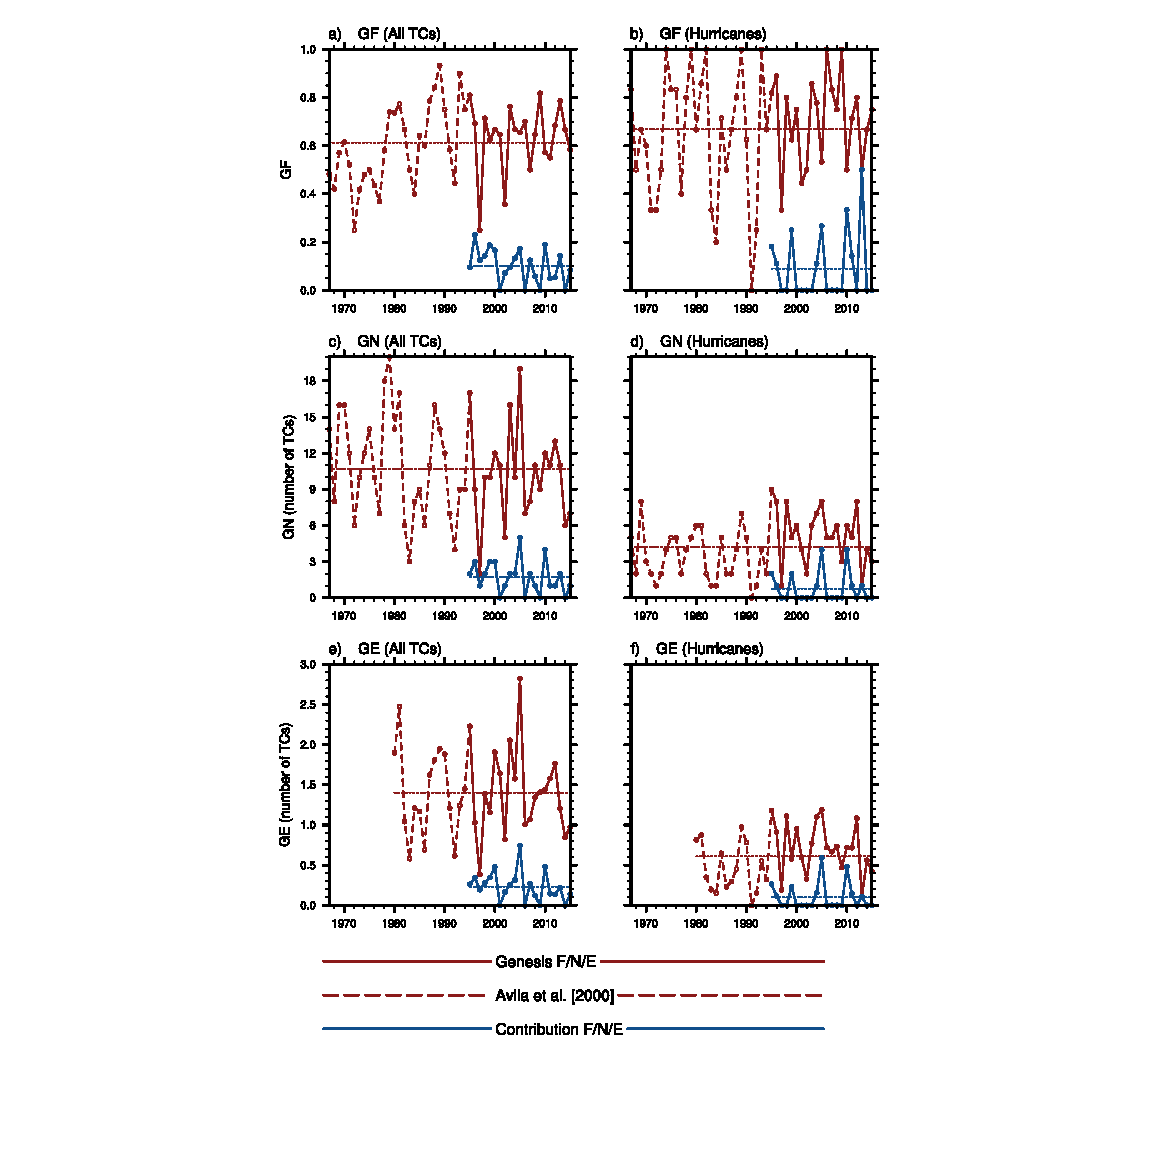
\includegraphics[trim={4cm 8.5cm 3cm 0cm},clip,width=\textwidth]{Chapter-1/figs/gfgnge_vs_year.eps}
\caption{Caption...}
\label{fig:gfgn}
\end{figure}

%--
\section{Background}
\label{sec:back}
%--

Background literature on topic

Possible citation in parentheses \citep{kiladis2006three} 

Possible citation in parentheses with text before or after also in parentheses \citep[e.g. ][ Figure 1]{kiladis2006three} 

Citation in text \citet{tomassini2017interaction}

%----------
\section{Open Questions and Theories}
\label{sec:que}
%----------

In this section I will present the open questions on the problem I am investigating. 

\subsection{Influence of AEWs on Convection}
\label{sec:QTaew-conv}

Background on theories

In summary we will attempt to address the following questions with regard to ...:
\begin{enumerate}
\item Question 1?
\item Question 2?
\item Question 3?
\end{enumerate}

\chapter{Gene Discovery through Plant Genome Environment Associations:
The Case for Enhanced Machine Learning Models of Soil Phosphorus Availability}
\label{chap-two}

\newrefsection

\section{Abstract}

\section{Background} 

Wild plants and crops show genetic adaptation to local soil conditions. 
In the high end of selection strength, maladapted individuals are not even able to survive extreme environments. 
This is the case of serpentine soils, which are very adverse to plant life, having alkaline pH, limiting amounts of nutrients like phosphorus, and elevated levels of heavy metals like nickel \citep{alexander2006}.
However, some populations of \textit{Mimmulus guttatus} are able to thrive there nonetheless. 
Using 2 independent mapping populations \citep{selby2018} were able to map a Quantitative Trait Locus (QTL) underlying survival in serpentine soils.
Furthermore, with common garden experiments, they isolated the genotypic effect of soil adaptation from water availability, exposure, and community composition \citep{selby2018}.
In less extreme cases, soil selective pressures do not result in death but penalize plant growth and yield.
For example, \citep{lasky2015-ar} found candidate \textit{Sorghum} adaptive loci to acid soils using Genome Environment Associations with topsoil pH in African traditional varieties. 
Later they were able to validate, in an independent \textit{Sorghum bicolor} inbred panel from the USA, the candidate SNPs by assessing their predictive value on seedling root growth in an acid substrate, where they contributed with a low but significant effect (Pearson $r \approx 0.3$) \citep{lasky2015-ar}. 

During domestication, maize has been selected for architectural root traits that increase resource acquisition in comparison to its wild relatives \citep{burton2013a,perkins2021}. When compared with teosinte, traditional Mexican maize varieties have a higher number of seminal roots \citep{burton2013a}, and this phenotype shows a pattern of local adaptation correlated with mean annual precipitation, and consequently to drought \citep{mclaughlin2023}.
Given the continuous selection for yield in industrial agriculture, optimal conditions for crops are rarely met in natural soils, and elite corn hybrids usually require fertilizer and other artificial inputs for maximal output. 

Low soil phosphorus availability for crops is the rule rather than the exception at the global scale \citep{mcdowell2023,batjes2019,lyons2023}. 
And Mexican soils are no different. 
I calculate a median topsoil available phosphorus concentration of 3.5 ppm (mg/kg) with 79\% of the natural soils samples below 10 ppm \citep{paz-pellat2018} \autoref{fig::obeserved_PHOS} (see Methods). 
For comparison, the minimal US test phosphorus recommendations for corn start at 15 ppm \citep{lyons2023}.

Soil tests cannot precisely tell the exact available amount of phosphorus for plants, instead, they provide an estimate of what the plant might acquire \citep{beegle2002}. 
These estimations are based on extensive yield trials at a range of soil phosphorus test values in multiple types of soils, which allows the construction of calibration curves and the assessment of critical values with the ultimate goal of giving farmers valid practical recommendations at the local level\citep{culman2023, dodd2005, beegle2002}. 
The most common extractants for phosphorus tests are Bray-1 (aka Bray-Kurtz)\citep{bray1945}, Meilich-3 \citep{mehlich1984} and Olsen \citep{olsen1954}.
The first two work best for neutral and acid soils and the last one correlates better with plant yield in alkaline calcareous soils \citep{culman2020}.
Due to differences in soils and policies between states, there is no single standard for soil phosphorus tests in the US \citep{lyons2023}.
The minimum soil test phosphorus recommendations for crop optimal yield in the USA, vary between 15 to 31 ppm depending on test and state \citep{lyons2023}, with yield trials of 10 ppm Bray-1 phosphorus producing relative yield losses up to 50\% \citep{dodd2005}. In contrast to the US, the Mexican government has adopted a straightforward approach. 
The reported available phosphorus for \citep{paz-pellat2018}, hereafter referred to as PHOS, corresponds to Bray-1 test phosphorus for neutral and acid soils (aka Bray-Kurtz)\citep{bray1945} and to Olsen test phosphorus for basic soils \citep{olsen1954}.

However, I find that global models of plant-available phosphorus, and other phosphorus parameters, have a very low prediction value in Mexico, with the Pearson correlation between these experimental \citep{paz-pellat2018} and the predicted values below $r=0.1$ \autoref{fig::phoscorrelation}.

For this reason, I use digital soil mapping based on machine learning techniques to predict the distribution of plant soil available phosphorus

\begin{figure}[!ht]
\centering
\includegraphics[width=0.9\linewidth]{Chapter-2/figs/obeserved_PHOS.png}
\caption[Experimental values for topsoil plant available phosphorus (PHOS) in Mexico]{\textit{\textbf{Experimental values for topsoil plant available phosphorus (PHOS) in Mexico.}} \\\hspace{\textwidth} 
\textbf{(A)} Geographical distribution of sampled soil profiles. For acid and neutral soils ($\text{pH} \leq 7$) the reported PHOS value corresponds to Bray-1 phosphorus. For basic soils Olsen phosphorus is reported as PHOS  \citep{paz-pellat2018}.
\textbf{(B)} Available phosphorus per WRB soil group determination method, \textit{left:} observed WRB determination in the field for INEGI reference profiles, \textit{right:} assignation of dominant soil in the corresponding map unit (polygon) in \citep{inegi2013}. The downward triangle points to Andosol group soils}
\label{fig::obeserved_PHOS}
\end{figure}
\clearpage

 
%% \begin{figure}[!ht]
%% \centering
%% \includegraphics[width=\linewidth]{Chapter-2/figs/WRB_Pret.png}
%% \caption[Phosphorus Retention Potential For Maize Traditional Varieties in Latin America and the Caribbean]{\textbf{\textit{Phosphorus Retention Potential For Maize Traditional Varieties in Latin America and the Caribbean.}}
%% Based on \citep{batjes2011}.  Each soil unit corresponds to a mineral descriptor, e.g. Acrisol soil units can be gleyic, humic, orthic, or plinthic. Ferric acrisols have very low phosphorus solubility potential (first column), the other three acrisol units have low solubility (second column). The soil groups with predominantly High and Very High solubility are Ferralsols, Andosols, Acrisols, and Nitosols.}
%% \label{fig::WRB_Pret}
%% \end{figure}
%% \clearpage

\section{Methods}
\subsection{Building and Validating a Model for Plant Available Phosphorus Distribution in Mexico}

To find associations between plant-available soil phosphorus and the genetic diversity of maize traditional varieties, I started by compiling public datasets on global phosphorus distribution. 
Because of its high resolution and interpretability, I intended to use the Olsen \citep{olsen1954} phosphorus predictions by \citep{mcdowell2023}.
However, the training data for this model contained no experimental Olsen determinations for Mexico, just 32 data points regressed from Bray-1 or resin values. 

In addition to \citep{mcdowell2023}, I searched for other datasets and parameters that could be correlated to experimental measures of plant-available phosphorus in soils. These included total phosphorus from \citep{hexianjin2022}, labile and total phosphorus from \citep{yang2013}, phosphorus by Bray-1, Olsen and Mehlich \citep{mehlich1984} methods, New Zealand phosphorus retention from \citep{shangguan2014} and NP limitation from \citep{du2020}.

Knowing that these models relied on a poor sampling Latin America, I decided to use as a benchmark the published experimental phosphorus data from the Instituto Nacional de Estadística y Geografía \citep{paz-pellat2018} of georeferenced soil profiles collected between 1969 to 2006.
This set contained topsoil phosphorus measurements as extractable phosphorus concentration in ppm [mg/kg] for 13092 gelolocalized soil profiles, divided into 8325 datapoints for  Olsen phosphorus (soils $\text{pH} > 7$) and 4767 data points for Bray phosphorus  (soils with $\text{pH} \leq 7$) for Mexico. 

For investigating the phosphorus distribution among different soil types according to WRB taxonomy \citep{wrb2014},  I used the field determinations of WRB soil group for the INEGI Serie II data \citep{inegi2013} and corresponding interpretation \citep{inegi2011,inegi2009} that matched both in profile identifier and geolocation within a 150m error. 

Then I followed the random forest based methodology for soil predictive mapping developed by \citep{hexianjin2022} because of its demonstrated prediction value for total phosphorus, interpretability and computational time savings in comparison with the more onerous 150 input predictor models of \citep{hengl2019} or \citep{mcdowell2023}. 
Here I used the maps for 16 predictors of available phosphorus, improving data cleanup and resolution where possible.
The predictors were as follows: Mean Annual Temperature and Mean Annual Precipitation from BioClim 2.0 at 10 km resolution \citep{fick2017}; WRB soil groups at 10 km and pH, soil organic carbon, bulk density at 250 m resolution, from SoilGrids 250 \citep{hengl2019,hengl2017,wrb2022,scheffe2015}, USDA taxonomy order from OpenLandMap at 250 m, biomes fom Resolve Ecoregions \citep{dinerstein2017} at 10 km, Mean Annual Net Primary Production from MODIS \citep{running2015a} at 250 m, elevation at 15m resolution from INEGI CEM 3.0 \citep{inegi2019}, slope at 1 km from EarthEnv \citep{amatulli2018}, soil depth at 10 km from Land-Atmosphere Interaction Research Group \citep{shangguan2017}, and lithology from GLiM rasterized at 10 km resolution\citep{hartmann2012}.
% (details on Supplementary file S1).
All coordinates were matched to WGS84 latitude longitude for extraction of values from each raster using the custom R scripts.

I ran 15 simple random forest models with these 16 predictors and a single response variable using the R library `randomForest` \citep{liaw2002}. 
I used as output a synthetic variable I called PHOS consisting in the union of those two sets of observations, i.e. the PHOS parameter is a measure of phosphorus availability in the soil that corresponds to Bray I extractable phosphorus if the soil $\text{pH} \leq 7$ and to the Olsen extractable phosphorus if the soil $\text{pH} > 7$. 
I followed the code used by \citep{hexianjin2022}  with 3 random variables selected at each decision node, 500 trees per model, $70\%$ training, $30\%$ testing data a 5-fold cross-validation at each step.
The predictive value of the model is measured as the Pearson correlation between the observed experimental values of available phosphorus concentration and the prediction from the random forest in the test data. 
Cross-validation was used to measure the contribution of each predictor to the model by removing it from the model and measuring the resulting change in the mean standard error of the prediction as a percentage. 
Additionally, I ran an ensemble model based on the 15 outputs of the simple random forest model to see if it would increase predictive values in the test data.

Although I increased the correlation between observations and predictions using the ensemble model up to 0.99, I did not observe an improvement in the test predictions worthy of the more complicated model.

% The POINTDATA needed additional matching in resolution and projection for making a raster prediction at 10 km resolution. So in  I used  \href{https://github.com/sawers-rellan-labs/grassGEA}{a series of custom $`R`$ language scripts} based on the `raster`, `gdal`, `sp` and `stars` libraries for obtaining 15 10km ($0.8883 \times 0.9993$ decimal degrees) latitude longitude WGS84 rasters. This dataset will be referred as MAPDATA.

\subsection{Gene Environment Association}
I used 495,755 SNPs genotyped in 2182 georeferenced maize traditional varieties \citep{romero_navarro2017-cn} to make genome environment associations with the PHOS parameter.
With these, I used a linear mixed model correcting for 10 principal components of the kinship matrix as correction for population structure as fixed effects, in addition to using the kinship matrix itself in the random effects with GEMMA (version: 0.98.3) \citep{vogt2022} as executed by vcf2gwas software (version: 0.8.7) \citep{zhou2012}. Bonforren correction was use to establish the statistical significance threshold.

For comparison, I calculated the fixation index $F_st$ between the deciles at the end of PHOS distribution. 

\section{Results}

\subsection{Random Forest Model of Olsen and Bray Phosphorus Improves Accuracy of Soil Available Phosphorus Estimation in  Mexico}
After building on the work of \citep{hexianjin2022} and \citep{mcdowell2023}, I increased the predictive value of the soil mapping models for Olsen and Bray extractable phosphorus in  Mexico. The the Pearson correlation $r$ from 0.08 to 0.37 (0 and 0.14 $R^2$) for observed and predicted values of plant available phosphorus (PHOS) compared to \citep{mcdowell2023}. PHOS prediction value is well bellow those used for species distributio models, like  mean annual temperature,$R^2$ = 0.98 \citep{fick2017}).
However, our model improves prediction for in Mexico compared to previous global models \cite{mcdowell2023} and a comparable model of plant available phosphorus in  Africa $R^2$ = 0.12  \citep{hengl2017a} 
Appart from the predictive value,  the relative importance of predictors in our models is congruent with the chemical understanding of how phosphorus goes into soil solution.
Phosphorus in solution depends on pH and soil mineralogy, while the total amount of phosphorus in non-fertilized soils should depend mostly on parent material and organic mater fractions.
Thus the random forest predictor importance as measured by \%IncMSE in our small model is easier to understand than models including multiple multispectral vegetation indices and climate variables \citep{mcdowell2023}.
This leads us to conclude that we have a more parsimonious model that has better prediction value and better interpretability.

% In addition to this we see good overlap with the training data set for both Africa and LAC (Figure 1C) (MANOVA test), which allows us to make reasonable interpolations. A similar approach increased the total phosphorus predictive value as well from 0.81 to 0.91 (0.65 and 0.81 $R^2$), marginally improving previously reported data for Africa \citep{hengl2017a}, where we expect even less over-fit because of the better sampling and increased mixing of data points in the predictor space.

% Not only our model shows acceptable and improved internal consistency, but it has increased correlations with other reported measurements of available P. For example for the LAC pixels corresponding to the Hou sampling of Hedley available phosphorus the correlation between our Olsen is 0.5  and Bray is 0.4. For the Africa isDASOIL \citep{miller2021b} extractable phosphorus is 0.4.
% At the level of continental and global models our Bray and Olsen predictions have high correlation with McDowell Olsen at the global scale but not in the southern hemisphere, with the predicted water soluble phosphorus in Africa \citep{miller2021b,hengl2017a}and low correlations with previous raster values based on heuristics models like \cite{shangguan2014}, \cite{yang2013} and\cite{batjes2011} retention probabilities.


\begin{figure}[!ht]
\centering
\includegraphics[width=0.9\linewidth]{Chapter-2/figs/WRB_inegi2013map.png}
\caption[WRB Soil Group Classification for Mexican soils according to INEGI]{\textit{\textbf{WRB Soil Group Classification for Mexican soils according to INEGI.}} \\\hspace{\textwidth}
\textbf{(A)} Reference soil profiles ($n \approx 4000$) \citep{inegi2013}.
\textbf{(B)} 1:250000 map prediction for the dominant WRB soil group \citep{inegi2015}
\textbf{(C)} Andosols predominate in the Transmexican Volcanic Belt at high altitudes and are frequent in the Sierra Nevada de Chiapas y Guatemala, collection areas for the Andosol Introgression Resource population \autoref{chap-four}}
\label{fig::WRB_inegi2013map}
\end{figure}
\clearpage


\begin{figure}[!ht]
\centering
\includegraphics[width=\linewidth]{Chapter-2/figs/WRB_inegi_soilgrids.png}
\caption[Comparison between INEGI and SoilGrids WRB soil Classification Maps]{\textit{\textbf{Comparison between INEGI and SoilGrids WRB soil Classification maps.}} \\\hspace{\textwidth}
\textbf{(A)} INEGI 1:250000 map dominant soil prediction sorted by AUROC, total count above the bar. From Histosols to the right misclassifications are more common than correct classifications. For Lixisisols, Cambisols, Acrisols and Plinthosols the most frequent prediction does not match the observed soil group.
\textbf{(B)}  INEGI 1:250000 map dominant soil prediction in absolute frequency scale (count), same as the number of top of A bars.
\textbf{(C)} Soilgrids 10 km WRB dominant soil prediction. Downscaled resolution from 250 m.
\textbf{(D)} Soilgrids 250 WRB dominant soil prediction, it  has more missing data and underpredicts Andosols}
\label{fig::WRB_inegi_soilgrids}
\end{figure}
\clearpage


\begin{figure}[!ht]
\centering
\includegraphics[width=0.65\paperwidth]{Chapter-2/figs/PHOS_correlation.png}
\caption[Pearson correlations (r) between experimental soil available phosphorus in Mexico (PHOS) and predicted phosphorus parameters from global models]{\textit{\textbf{Pearson correlations (r) between experimental soil available phosphorus in Mexico (PHOS) and predicted phosphorus parameters from global models.}} Observed values for lon : longitude, lat: latitude, ele: elevation in \citep{inegi2013}, and clay: clay content, pH, and PHOS: plant available phosphorus in \citep{inegi2013}. Predicted probabilities for Lo: Low, Mo: Moderate, Hi: High, and VH: very high phosphorus retention potential soil classes according to \citep{batjes2011}; predicted
stp10: total phosphorus from \citep{hexianjin2022}, lab: labile and tot: total phosphorus from \citep{yang2013}, phosphorus by Bray, Olsen and Mehlich methods and New Zealand phosphorus retention  from \citep{shangguan2014}; and predicted NPlim: Nitrogen Phosphorus limitation from \citep{du2020}. } 
\label{fig::phoscorrelation}
\end{figure}
\clearpage

\begin{figure}[!ht]
\includegraphics[width=0.9\linewidth]{Chapter-2/figs/marginal_dependencies.png}
\caption[Marginal Dependencies of PHOS. Distribution of pH and elevation by  WRB soil groups] {\textit{\textbf{Marginal Dependencies of PHOS. Distribution of pH and elevation by  WRB soil groups.}} \textbf{(A)} \textit{Top:} Grey circles: experimental values for natural Mexican soils. Spline tendency in blue with confidence interval in grey.  A local maximum of predicted PHOS is found at $\text{pH} = 7.25$, while the global maximum is found at $\text{pH}> 9$. There is a tendency of decreased PHOS with clay content (\%), and there is an increase of PHOS at elevations $> 3000$ masl.
\textit{Bottom:} Zoom on median values, for predictor deciles and 1000 bootstrap confidence intervals. Dashed line is the median value for all samples.
\textbf{(B)} Distribution of pH and elevation by imputed WRB  soil
groups. 
Imputed WRB samples are the union of experimental reference WRB taxonomy determinations, and predictions of dominant soil group from \citep{inegi2013} (see \autoref{fig::obeserved_PHOS} B).
Andosols are typical acid soils mostly found at elevations above 2000 masl.}
\label{fig::marginal_dependencies}
\end{figure}
\clearpage



\begin{figure}[!ht]
\centering
\includegraphics[width=0.9\linewidth]{Chapter-2/figs/rf_validation.png}
\caption[Random forest model validation for soil  available phosphorus PHOS in Mexico]{\textit{\textbf{Random forest model validation for soil  available phosphorus PHOS in Mexico.}}\\\hspace{\textwidth} 
\textbf{(A)} Correlation between observed and predicted available phosphorus in linear (top) and logarithmic (bottom) scales.
The model is overfitted as it has far better predictive value over training $r=0.8$ rather than testing $r=0.4$ data.
\textbf{(B)} Predictor contribution calculated as mean square error difference (\%) after removing it from the model.}
\label{fig::rfvalidation}
\end{figure}
\clearpage





\begin{figure}[!ht]
\centering
\includegraphics[width=\linewidth]{Chapter-2/figs/predicted_PHOS.png}
\caption[Predicted Available Phosphorus for Mexican Traditional Maize Varieties]{\textit{\textbf{Predicted Available Phosphorus for Mexican Traditional Maize Varieties.}}
\\\hspace{\textwidth}
\textbf{(A)} Geographical distribution for 2182 traditional varieties from the FOAM panel \citep{romero_navarro2017-cn}
\textbf{(B)} Comparison of topsoil phosphorus in 13092 soil profiles \citep{paz-pellat2018} with the predictions for the FOAM panel.}
\label{fig::pointpred}
\end{figure}
\clearpage

\subsection{Genome Environment Associations Point to Candidate Genes for Adaptation to Diverse Soil Phosphorus Availability Conditions}

Now with the best model of plant available phosphorus for Mexican soils  I  proceeded to look for Genome Environment Associations in Traditioal maize varieties in Mexico.

\subsection{Discussion}

% \begin{figure}[b]
% \centering
% \includegraphics[width=\linewidth]{Chapter-2/figs/PHOS_mlm.png}
% \caption[]{}
% \label{fig:PHOS_mlm}
% \end{figure}
\clearpage

%\addtocounter{figure}{-1}
\begin{figure} [t!]
\includegraphics[width=0.8\linewidth]{Chapter-2/figs/PHOS_mlm.png}
\caption[Linear Mixed Model Association between Maize Genetic Variants and Soil Available Phosphorus in Mexican Traditional Varieties]{\textit{\textbf{Linear Mixed Model Association between Maize Genetic Variants and Soil Available Phosphorus in Mexican Traditional Varieties.}}
%% \\\hspace{\textwidth}
\textbf{(A)}  QQ-plot showing genomic inflation factor of p-values of the LMM association
\textbf{(B)} Corresponding Manhattan plot 
\textbf{(C)} Allelic substitution "effect" of rs86953444 on PHOS.
\textbf{(D)} Allele frequency cline.
\textbf{(E)} Multinomial logistic regression of Genotype Frequency on PHOS.
\textbf{(F)} Genomic context of rs86953444 pointing to an auxin response transcription factor candidate \textit{ZmARF12}.
\textbf{(G)} \textit{ZmNAC82} kernel expression.
\textbf{HG)} \textit{ZmARF12} kernel expression.
}
\end{figure}
\clearpage

\begin{figure}[!ht]
\centering
\includegraphics[width=\linewidth]{Chapter-2/figs/PHOS_Fst.png}
\caption[Fst based Association between Maize Genetic Variants and Soil Available Phosphorus in Mexican Traditional Varieties]{\textit{\textbf{ $\boldmath{F_{st}}$ based Association between Maize Genetic Variants and Soil Available Phosphorus in Mexican Traditional Varieties.}}
% \\\hspace{\textwidth} 
\textbf{(A)} Genome $F_\text{st}$ distribution   showing differentiation between extreme deciles of PHOS $<9$ and $>20$ ppm. Three bars are shown for comparison, weighted genomewide mean $F_\text{st}$ \citep{hufford2013-gs} between blue: Mexican maize traditional varieties (TV) and tesosinte (\textit{mexicana} and \textit{parviglumis});  red: TV vs improved germplasm; and dashed: maximum $F_\text{st}$.
\textbf{(B)} Corresponding Manhattan plot.
\textbf{(C)} Genotype frequencies at the SNP with maximal differentiation PZE0558576811
\textbf{(D)} Allelic substitution "effect" on PHOS \textbf{(E)}Allele frequency cline.
\textbf{(F)} Multinomial Logistic Regression of Genotype Frequency on PHOS.
\textbf{(G)} Gneomic contest of PZE0558576811 pointing to a transcription factor candidate  Zm0001eb22747 \textbf{(H)} Zm0001eb22747 kernel expression.
 }
\label{fig::PHOS_Fst}
\end{figure}
\clearpage


\printbibliography[heading=subbibnumbered, title=References]
\chapter{Results 1}

bla bla bla ...
%%---------------------------------------------------------------------------%%
% Appendices
%\ensureoddstart
\restoregeometry
\appendix
%\newgeometry{margin=1in,lmargin=1.25in,footskip=\chapterfootskip, includehead, includefoot}

% Can remove or add
% \chapter{\hpc Supplementary Material}
\begin{table*}[h!]
\centering
\caption{Pairwise $C_{hyper}$ statistic for population comparisons.}
\begin{tabular}{@{}llll@{}}
\toprule
population 1 & population 2 & $C_{hyper}$   & $p$  \\ \midrule
US   & MH   & 3.82 & 1.11E-04 \\
US   & GH   & 6.17 & 8.00E-10 \\
MH   & GH   & 4.37 & 1.24E-05 \\
US   & AN   & 3.51 & 3.37E-04 \\
MH   & AN   & 2.73 & 4.43E-03 \\
GH   & AN   & 3.16 & 1.16E-03 \\ \bottomrule
\end{tabular}
\label{tab:C_hyper}
\end{table*}

% \hspace{2em}
\begin{table*}[h]
\centering
\caption[Selection outliers simultaneously detected in PBE and pcadapt analysis]{\textbf{Selection outliers simultaneously detected in PBE and pcadapt analysis}. These phosphoglycerolipid metabolism genes are in the top 5\% of Mexican highlands PBE, and are also in the top 5\% of significance ($-log_{10}(P)$) for the association with \textit{pcadapt} PC1 (elevation correlated principal component).  Further populations where the gene is an outlier for PBE are listed as well, maximum PBE  population is highlighted in bold.
}
\resizebox{\textwidth}{!}{%
\begin{tabular}{@{}ll@{ }l@{ }l@{ }lllrrll@{}}
\toprule
               & \multicolumn{5}{c}{\textbf{PBE}}                             & \multicolumn{3}{c}{\textbf{pcadapt}} &                                                                                                        &                                                                                                  \\
\cmidrule(lr){2-6} \cmidrule(lr){7-9}  
Gene           & \multicolumn{4}{c}{Outlier Population}      & Max  & chr   & bp          & \textbf{$-log_{10}(P)$}   & Description                                                                                            & Example Pathway                                                                                  \\
\midrule
Zm00001d009280 &             & \textbf{MH} &    &             & 0.55 & 8     & 50352267    & 207.55                    & \begin{tabular}[c]{@{}l@{}}phosphoethanolamine\\ N-methyltransferase\end{tabular}                      & \begin{tabular}[c]{@{}l@{}}superpathway of phospholipid \\ biosynthesis II (plants)\end{tabular} \\
Zm00001d046915 &             & MH          & GH & \textbf{AN} & 0.81 & 9     & 107790977   & 138.64                    & AMP-dependent synthetase                                                                               & phosphatidylcholine acyl editing                                                                 \\
Zm00001d014425 &             & \textbf{MH} & GH &             & 1.19 & 5     & 44991886    & 134.29                    & Glycerol-3-phosphate acyltransferase                                                                   & \begin{tabular}[c]{@{}l@{}}superpathway of phospholipid\\ biosynthesis II (plants)\end{tabular}  \\
\underline{Zm00001d039542} & US          & \textbf{MH} & GH &             & 1.01 & 3     & 8542287     & 110.28                    & \begin{tabular}[c]{@{}l@{}}Phospholipase A1-Igamma1 chloroplastic\\ HPC1\end{tabular}                  & phosphatidylcholine acyl editing                                                                 \\
\underline{Zm00001d017584} & \textbf{US} & MH          & GH & AN          & 0.86 & 5     & 195455216   & 99.31                     & \begin{tabular}[c]{@{}l@{}}Lysophospholipid acyltransferase 1\\ ZmLPCAT1\end{tabular}                  & phosphatidylcholine acyl editing                                                                 \\
Zm00001d040629 & US          & MH          & \textbf{GH} & AN          & 1.80 & 3     & 55167339    & 85.67                     & Lysophospholipid acyltransferase LPEAT1                                                                &                                                                                                  \\
Zm00001d043267 & \textbf{US} & MH          &    &             & 1.11 & 3     & 190926980   & 68.94                     & \begin{tabular}[c]{@{}l@{}}acyl-CoA:1-acyl-sn-glycerol-3-phosphate \\ 2-O-acyltransferase\end{tabular} & \begin{tabular}[c]{@{}l@{}}superpathway of phospholipid\\ biosynthesis II (plants)\end{tabular}  \\
Zm00001d043263 &             & \textbf{MH} & GH & AN          & 1.02 & 3     & 190792965   & 66.70                     & Diacylglycerol kinase 5                                                                                & \begin{tabular}[c]{@{}l@{}}phosphatidate metabolism,\\ as a signaling molecule\end{tabular}      \\ \bottomrule
\end{tabular}%
}
\label{tab:Sup:top_candidates}
\end{table*}
\clearpage

\begin{figure*}[t]
\begin{center}
\includegraphics[width=\linewidth]{Sup_Figures/Sup_Fig_1.png}
\caption[Cluster analysis of lipidomics data]{\textbf{Cluster analysis of lipidomics data.} Representative species from each cluster were used for $Q_{ST}$-$F_{ST}$ analysis}
\label{figure:Sup:lipid_clusters}
\end{center}
\end{figure*} 
\clearpage

\begin{figure*}[t]
\begin{center}
\includegraphics[width=\linewidth]{Sup_Figures/Sup_Fig_2.png}
\caption[Effects of QTLs at chromosome 3 @8.5 Mb]{\textbf{Effects of QTLs at chromosome 3 @8.5 Mb} \textbf{(a-d)} Effect for individual PC \textbf{(e-f)} and LPC species
\textbf{(g-r)} The 12 most significant peaks for PC/LPC ratios} 
%\label{QTL_effect_sp}
\label{figure:Sup:QTL_effect_sp}
\end{center}
\end{figure*}  
\clearpage

\begin{figure}[t]
\begin{center}
\includegraphics[width=\linewidth]{Sup_Figures/Sup_Fig_3.png}
\caption[Phospholipase activity in maize.]{\textbf{Phospholipase activity in maize.} \textbf{(A)} Genomic location of genes encoding proteins with predicted phospholipase A1 activity. 
\textbf{(B)} Site of action of the different types of phospholipases.
\textbf{(C)} Expression levels from B73 leaves for genes in the 7.9--10 Mb QTL interval of chromosome 3. Data from \cite{stelpflug2016-vr}
\textbf{(D)} Effect sizes of PC/LPC levels at RILs homozyzogous for B73, PT or heterozygous at the QTL qPC/LPC3@8.5.
}
\label{figure::Sup:HPC1_misc}
\end{center}
\end{figure} 
\clearpage

\begin{figure*}[t]
\begin{center}
\includegraphics[width=\linewidth]{Sup_Figures/Sup_Fig_4.png}
\caption[Phospholipase expression in temperate inbred lines.]{\textbf{Phospholipase expression in temperate inbred lines.} \textbf{A)} Expression levels in B73 of genes encoding enzymes with predicted phospholipase A1 activity across different tissues. \hpc is indicated in blue. 
Data from \cite{stelpflug2016-vr}.
\textbf{B)}  and \textbf{C)}\hpc and \textit{ZmLPCAT1} expression levels in the temperate inbred lines B73, Mo17, OH43, and PH207 under cold and control conditions. Values taken from \cite{waters2017-nat}).
}
\label{figure:Sup:B73_expression}
\end{center}
\end{figure*} 
\clearpage

\begin{figure}[t]
\begin{center}
\includegraphics[width=0.8\linewidth]{Sup_Figures/Sup_Fig_5.png}
\caption[Subcellular localization of HPC1 in \textit{Nicotiana benthamiana} epidermal leaf cells.]{\textbf{Subcellular localization of HPC1 in \textit{Nicotiana benthamiana} epidermal leaf cells.}   
CTP.HPC1-GFP, corresponding to the first 52 amino acids HPC1, were fused to GFP. 
Three constructs for various subcellular compartments were used as control; cytoplasm (C-GFP), nucleus (N-GFP), and chloroplast (P-GFP). All reporters were under the control of the cauliflower Mosaic Virus (CaMV) 35S promoter. The white arrows show chloroplast and nucleus.
} 
\label{figure:Sup:HPC1_organelle}
\end{center}
\end{figure} 
\clearpage

\begin{figure*}[t]
\begin{center}
\includegraphics[width=\linewidth]{Sup_Figures/Sup_Fig_6.png}
\caption[Recombination at the \hpc promoter in the B73 x PT segregating population.]{\textbf{Recombination at the \hpc promoter in the B73 x PT segregating population.} \textit{Overview (top)} 1419 bp global alignment of Sanger sequences from B73 and 5 RILs (B035, B052, B042, B021 and B122). At variant positions B042 shows B73 genotype (grey) up to alignment position 430, and PT genotype (red) from 789 downstream. We infer that there is  a recombination breakpoint between -493 and -136 bp upstream the translation start codon of B042.
HapMap track shows HapMap2.7 SNPs used for Linkage Disequilibrium calculations in MaizeSNPDB as in Figure 5. The 5' LD block spans the upstream intergenic region, including two ATAC-seq chromatin accessibility peaks (one included in this fragment), and up to 364 bp of \hpc coding sequence. 
Then there is a LD break, and a downstream 3' LD block (not included in these sequences). 
\textit{TIR-TE} terminal inverted repeat transposable element. 
B73 ATAC-seq: narrow peak showing chromatin accessibility in leaf tissue \cite{ricci2019-zj}.
\textit{Base pair detail (bottom)} B73 and and PT nucleotide alleles are marked in grey and red respectively.
Coordinate numbers on top of both views are global alignment positions.
}
\label{figure:Sup:hpc1_promoter}
\end{center}
\end{figure*}
\clearpage

\begin{figure*}[t]
\begin{center}
\includegraphics[width=0.8\linewidth]{Sup_Figures/Sup_Fig_7.png}
\caption[Effects of the \textit{hpc1\textsuperscript{CR}} allele.]
{\textbf{Effects of the \textit{hpc1\textsuperscript{CR}} allele.}
\textbf{(A)} Physical location of \hpc CRISPR mutant alleles. \textbf{(B)} log(PCs/LPCs) ratios of WT and the \hpc CRISPR mutant alleles. \textbf{(C)} Days to anthesis of the same plants shown in panel A.   
}
\label{figure:Sup:CRISPR_effect}
\end{center}
\end{figure*} 
\clearpage



\begin{figure*}[t]
\begin{center}
\includegraphics[width=\linewidth]{Sup_Figures/Sup_Fig_8.png}
\caption[\hpc alleles have phospholipase activity.]
{\textbf{\hpc alleles have phospholipase activity.}
\textbf{A} Schematic of the \hpc reaction of PC(18:2/18:2) (red) to
PC(0:0/18:2) (blue). 
\textbf{B} IR-MALDESI-MS mass spectra of the HPC1 reaction using the \textit{HPC1-PT} and \textit{HPC1-B73} alleles. The
experimental \textit{m/z} and mass measurement accuracy (MMA) is labelled below each
identification. 
Both protonated and sodiated adducts of PC(18:2/18:2) were measured. 
Each mass spectrum was averaged over 100 scans.}
\label{figure:Sup:MS_spectra}
\end{center}
\end{figure*} 
\clearpage

\begin{figure*}[t]
\begin{center}
\includegraphics[width=0.8 \paperwidth]{Sup_Figures/Sup_Fig_9.png}
\caption[Genome wide association of genotype by elevation by genotype interactions of days to anthesis.]{Genome wide association of genotype by elevation by genotype interactions of days to anthesis \textbf{(A)} and cob weight \textbf{(B)} using data from \cite{gates2019-xu}}.
\label{figure:Sup:GxE_scan}
\end{center}
\end{figure*} 
\clearpage

\begin{figure*}[t]
\begin{center}
\includegraphics[width=\linewidth]{Sup_Figures/Sup_Fig_10.png}
\caption[Alignment of HPC1-B73 and HPC1-PT.]
{\textbf{Alignment of HPC1-B73 and HPC1-PT.}
Green residues are those from the chloroplast transit peptide.
Blue resides are part of the Lipase3 domain. 
Magenta residues are the flap lid. 
Arrow denotes I211V mutation. “*” denotes matching sequence, “:” denotes conservation between groups with similar properties, “.” denotes conservation of groups with weakly similar properties.
Aminoacid sequence aligned with ClustalOmega.}
\label{figure:Sup:aa_alignment}
\end{center}
\end{figure*} 
\clearpage

\begin{figure*}[t]
\begin{center}
\includegraphics[width=\linewidth]{Sup_Figures/Sup_Fig_11.png}
\caption[Correlation between flowering time and expression of phospholipid-related genes.]
{\textbf{Correlation between flowering time and expression of phospholipid-related genes.} 
Gene expression was correlated to flowering time traits from aerial tissues in the 282 diversity panel. 
Data obtained from \citep{kremling2018-gn}.}
\label{figure:Sup:cor_heatmap}
\end{center}
\end{figure*} 
\clearpage

\begin{figure*}[t]
\begin{center}
\includegraphics[width=\linewidth]{Sup_Figures/Sup_Fig_12.png}
\caption[Predicted binding sites of ZCN8 align with binding sites of Arabidopsis FT.]
{\textbf{Predicted binding sites of ZCN8 align with binding sites of Arabidopsis FT.}
Shown are AutoDock Vina \cite{trott2010-su} ZCN8 - lipid docking interactions of a RoseTTAFold \cite{baek2021sci} model of ZCN8 PC 34:2 \textbf{(A)} and PC 36:2 \textbf{(B)} compared with the docking model of PC 36:2 \textit{Arabidopsis thaliana} FT \textbf{(C)} from \cite{nakamura2019-ht}. 
Docking was performed on an NMRBox server \cite{maciejewski2010bj}.
\textbf{(D)} Alignment of \textit{Arabidopsis thaliana} FT and \textit{Zea mays} ZCN8. 
Residues in blue are present in both docking site 1 and docking site 4 identified in \cite{nakamura2019-ht}. 
Residues in magenta are present only in docking site 1 while residues in green are present only in docking site 4. 
Symbols below the residues indicate level of alignment where * denotes complete alignment, : represents a conserved substitution, and . represents a semi-conserved substitution.}
\label{figure:Sup:Docking}
\end{center}
\end{figure*} 


\begin{figure*}[t]
\begin{center}
\includegraphics[width=\linewidth]{Sup_Figures/Sup_Fig_14.png}
\caption[ZCN8 binds to phosphatidylcholine.]
{ \textbf{ZCN8 binds to phosphatidylcholine}.
\textbf{(A)} Mass spectrum of ZCN8-SPOT yeast sample compared to the theoretical isotopic pattern of PC(34:2) at [M+H]\textsuperscript{+} \textit{m/z} 758.5694. The experimental \textit{m/z} and mass measurement accuracy (MMA) are labeled. The spectrum of ZCN8-SPOT is an average of 16 scans across the chromatographic peak of \textit{m/z} 758.5694.  
\textbf{(B)} Extracted ion chromatogram of \textit{m/z} 758.5694 from the PC(16:0/18:2) standard and ZCN8-SPOT yeast from two separate injections.  
\textbf{(C)s} MS\textsuperscript{2} fragmentation spectra comparison for \textit{m/z} 758.5694 from ZCN8-SPOT yeast and the PC(16:0/18:2) standard.
The comparison data between an authentic standard and ZCN8-SPOT yeast was acquired with the same lipid profiling method as described in the Materials and Methods section for the Thermo Scientific Orbitrap Exploris 480 mass spectrometer with the following modifications:  the injection volume was 10 $\mu$L, full scan spectra were acquired from \textit{m/z} 200 – 1000 and \textit{m/z} 758.5694 was included in the target mass
list for MS\textsuperscript{2} selection.}
\label{figure:Sup:ZCN8-PC}
\end{center}
\end{figure*}



% \chapter{Variables}

A summary of all variables is documented in Table \ref{tab:vars}.

\begin{longtable}{| l | l |}
\caption{A summary of common meteorological variables and their abbreviations in alphabetical order.}\label{tab:vars}\\
\hline 
Variable & Abbreviation \\
\hline
Arbitrary variable & $X$ \\
Absolute vorticity vector & $\vec{\eta}$ \\
Coriolis parameter & $f$ \\
Gas constant for dry air & $R$ \\
Geopotential & $\Phi$ \\
Geopotential height & $Z$ \\
Gravitational accelleration & $g$ \\
Horizontal wind vector & $\vec{V}$ \\
Isobaric vertical motion & $\omega$ \\
Latent heat of vaporization & $l_v$ \\
Meridional unit vector & $\hat{j}$ \\
Meridional wind & $v$ \\
Potential temperature & $\theta$ \\
Potential vorticity & $P$ \\
Pressure & $p$ \\
Relative vorticity vector & $\vec{\zeta}$  \\
Specific density & $\alpha$ \\
Specific heat capacity at constant pressure & $c_p$ \\
Temperature & $T$ \\
Time & $t$ \\
Three-dimensional wind vector & $\vec{U}$ \\
Vertical absolute vorticity & $\eta$ \\
Vertical unit vector & $\hat{k}$ \\
Vertical relative vorticity & $\zeta$ \\
Zonal unit vector & $\hat{i}$ \\
Zonal wind & $u$ \\
\hline
\end{longtable}

\restoregeometry

%%---------------------------------------------------------------------------%%

%%---------------------------------------------------------------------------%%
\backmatter

\end{document}